\chapter{Resource Usage}

This module monitors the resource usage in the network. This module is also responsible for detecting deadlock and 
implementing heuristic that avoids deadlock upto certain extent (more details in the following sections). 
  
\section{Resource usage graph}
This component is responsible 
for creating graph, that shows which train is using which resource(track or station) and waiting for 
which resource(if any). Pink node corresponds to train, blue corresponds to stations and green corresponds 
to track. If a train is occupying a resource (station or track), then we have an arrow from resource to train.
If a train is waiting for a resource to be freed, then we have the arrow from train to resource.

\begin{figure}[h]
    \centering
    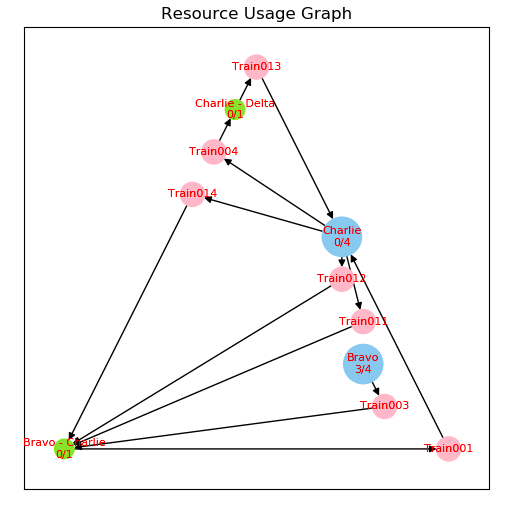
\includegraphics[width=0.65\textwidth]{resource}
    \caption{ Resource usage in the network.  }
    \label{image-myimage6}
\end{figure}

\section{Deadlock detection}
Simulator encounters deadlock if the next chosen move is
infeasible because $(i)$ vehicle $v$ finds all resources at the
next node occupied by other vehicles, and (ii) these other
vehicles can only release their current resources if they
move into the resource currently occupied by $v$. 
In the figure below, there are four trains at station Charlie, one train on track Delta-Charlie, trying to move to station Charlie 
and one train at track Charlie-Bravo, trying to move to station Charlie. Since no trains can move in this scenario, so it is in deadlock.

\begin{figure}[h]
    \centering
    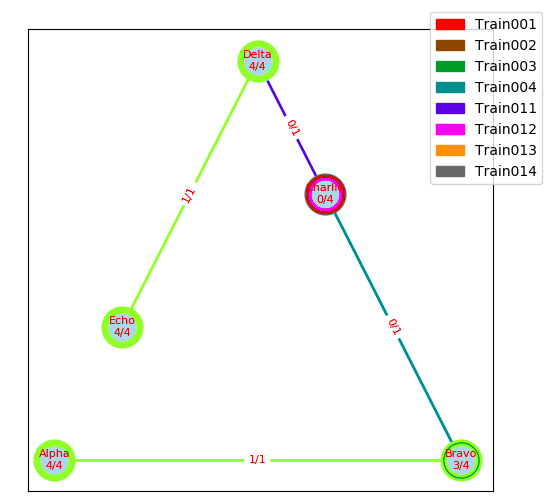
\includegraphics[width=0.65\textwidth]{deadlock}
    \caption{ Deadlock near station Charlie.  }
    \label{image-myimage6}
\end{figure}

In this simulator, each resource (station or track) is having multiple instances
(lines). If each resource have only one instance, then deadlock can be detected by cycle in resource 
usage graph. But since, each resource is having multiple instances, we have to use banker's algorithm to detect deadlock.
Once the deadlock is detected, simulation is terminated and huge negative reward is given.

\subsection{Banker's algorithm}

This algorithm is originally used to avoid deadlock. We are going to modify this to detect deadlock.
Here, trains are treated as processes and tracks or stations are treated as resources.
Let's $n$ be the number of processes (trains) and $m$ be the number of resource categories (number of stations and tracks in 
the network). The banker's algorithm relies on several key data structures:
\begin{enumerate}
\item $Available[m]$ indicates how many resources are currently available of each type.
\item $Max[n][m]$ indicates the maximum demand of each process of each resource.
\item $Allocation[n][m]$ indicates number of each resource category allocated to each process.
\item $Need[n][m]$ indicates the remaining resources needed of each type for each process. 
( Note that $Need[i][j] = Max[i][j] - Allocation[i][j]$   $\forall i, j$. )
\end{enumerate}

This algorithm determines if the current state of a system is safe, according to the following steps:
\begin{enumerate}
\item Let Work and Finish be vectors of length $m$ and $n$ respectively.
\begin{itemize}
\item Work is a working copy of the available resources, which will be modified during the analysis.
\item Finish is a vector of booleans indicating whether a particular process can finish (or has finished so far in the analysis).
\item Initialize Work to Available, and Finish to false for all elements.
\end{itemize}
\item Find an $i$ such that both $(A)$ $Finish[ i ] == false$, and $(B)$ $Need[i] < Work$. This process has not finished, but could with the given available working set. If no such i exists, go to step 4.
\item Set $Work = Work + Allocation[i]$, and set $Finish[i]$ to $true$. This corresponds to process $i$ finishing up and releasing its resources back 
        into the work pool. Then loop back to step 2.
\item If $finish[i] == true$  $ \forall i$, then the state is a safe state, because a safe sequence has been found.
\end{enumerate}

This algorithm is used to avoid deadlock. 
In our case $Available$ is the number of resource instances (lines 
on stations or tracks) free. $Allocated$ is the number of resource instance (lines on station or tracks) occupied 
by the train and $Requested$ is the resource instance requested by the train. 
If we use $Max = Allocated + Requested$, then above can be used to \textbf{detect deadlock} in the system.

\vspace{0.25cm}
Another important question is when to use deadlock detection algorithm. If use it very frequently 
then it's waste of computation as most the time system will not be in deadlock. If we use it very less
then system may be in deadlock for long time. So we have to find some middle ground. Here, we are currently checking deadlock
after every 20 units of time, it may be changed in the future. If the system is in deadlock, then 
simulation is terminated.

\vspace{5cm}
\section{Deadlock avoidance heuristic}
Multiple trains are running in the network. It is possible that multiple trains need action at a particular simulation time.
So we have to pick one of these trains, and take action (move or wait) corresponding to 
train. This is done using deadlock avoidance heuristic based on \cite{ARTICLE:2}.
Intuitively, pick the train which is in the most
congested resource first. The lower the number of free tracks
in a resource, the higher the congestion, and the earlier the
processing of a train occupying that resource. This way we can avoid deadlock upto certain extent.

\vspace{0.25cm}
This algorithm takes TRAINS\_NEEDING\_ACTION, which is a global variable consisting of all the trains
that need action at a particular time, as input and gives the name of the train that is suitable to 
take action as output. 

\subsection{Algorithm}
\begin{enumerate}

\item Find status of all trains (not yet started , running , at last station or completed journey) in  
    TRAINS\_NEEDING\_ACTION.
\item Remove all trains that have completed there journey since they don't need action and generate a warning in log 
    as such train should not be in TRAINS\_NEEDING\_ACTION.
\item If there is such a train which is on last station but not freed the resource, then return that train 
     and terminate the algorithm.
\item If there is a train that has not yet started and waiting to be put on first station, then 
     return that train and terminate the algorithm.
\item Now all the trains are running. Construct an array where each element is a tuple of size 5 and corresponds to trains in 
    the TRAINS\_NEEDING\_ACTION. Items in the tuple are : 
\begin{itemize}
\item Name of the train
\item Resource (track or station) it is occupying.
\item Congestion on the resource, given by number of occupied lines on the resource.
\item Priority of the resource, given by minimum of the priority of all trains on the resource. 
\item Priority of the train
\end{itemize}

\item Pick train which is on most congested resource. If there is one such unique train then return it and 
     and terminate the algorithm. If not, go to next step.
\item Out of trains chosen from step 6, pick train on resource with highest priority. If there is one train needing action on that resource 
     then return it and terminate algorithm. If not, go to next step.
\item Out of trains chosen from step 7, pick train with highest priority. If there are multiple train then choose any one randomly and return it. 
\end{enumerate}